\chapter{Задание входных данных для расчёта} \label{ch2}

Перед проведением расчёта в Ansys необходимо задать входные данные: геометрию рассматриваемой детали, конечно-элементную сетку и граничные условия.

Известно, что изделие изготовлено из конструкционной стали с модулем Юнга $E=200\text{ ГПа}$, коэффициентом Пуассона $\nu=0.3$ и плотностью \\ $\rho=7850\text{ кг/м}^3$.

\section{Построение CAD-модели изделия} \label{ch2:sec1}

3D-модель рассматриваемого изделия строим в Ansys DesignModeler. Сначала необходимо построить эскизы, на основе которых в дальнейшем с помощью функции Extrude будут получены полноценные 3D детали.

На рис. \ref{fig:sketch1} представлен эскиз хомута.

\begin{figure}[H] 
	\center
	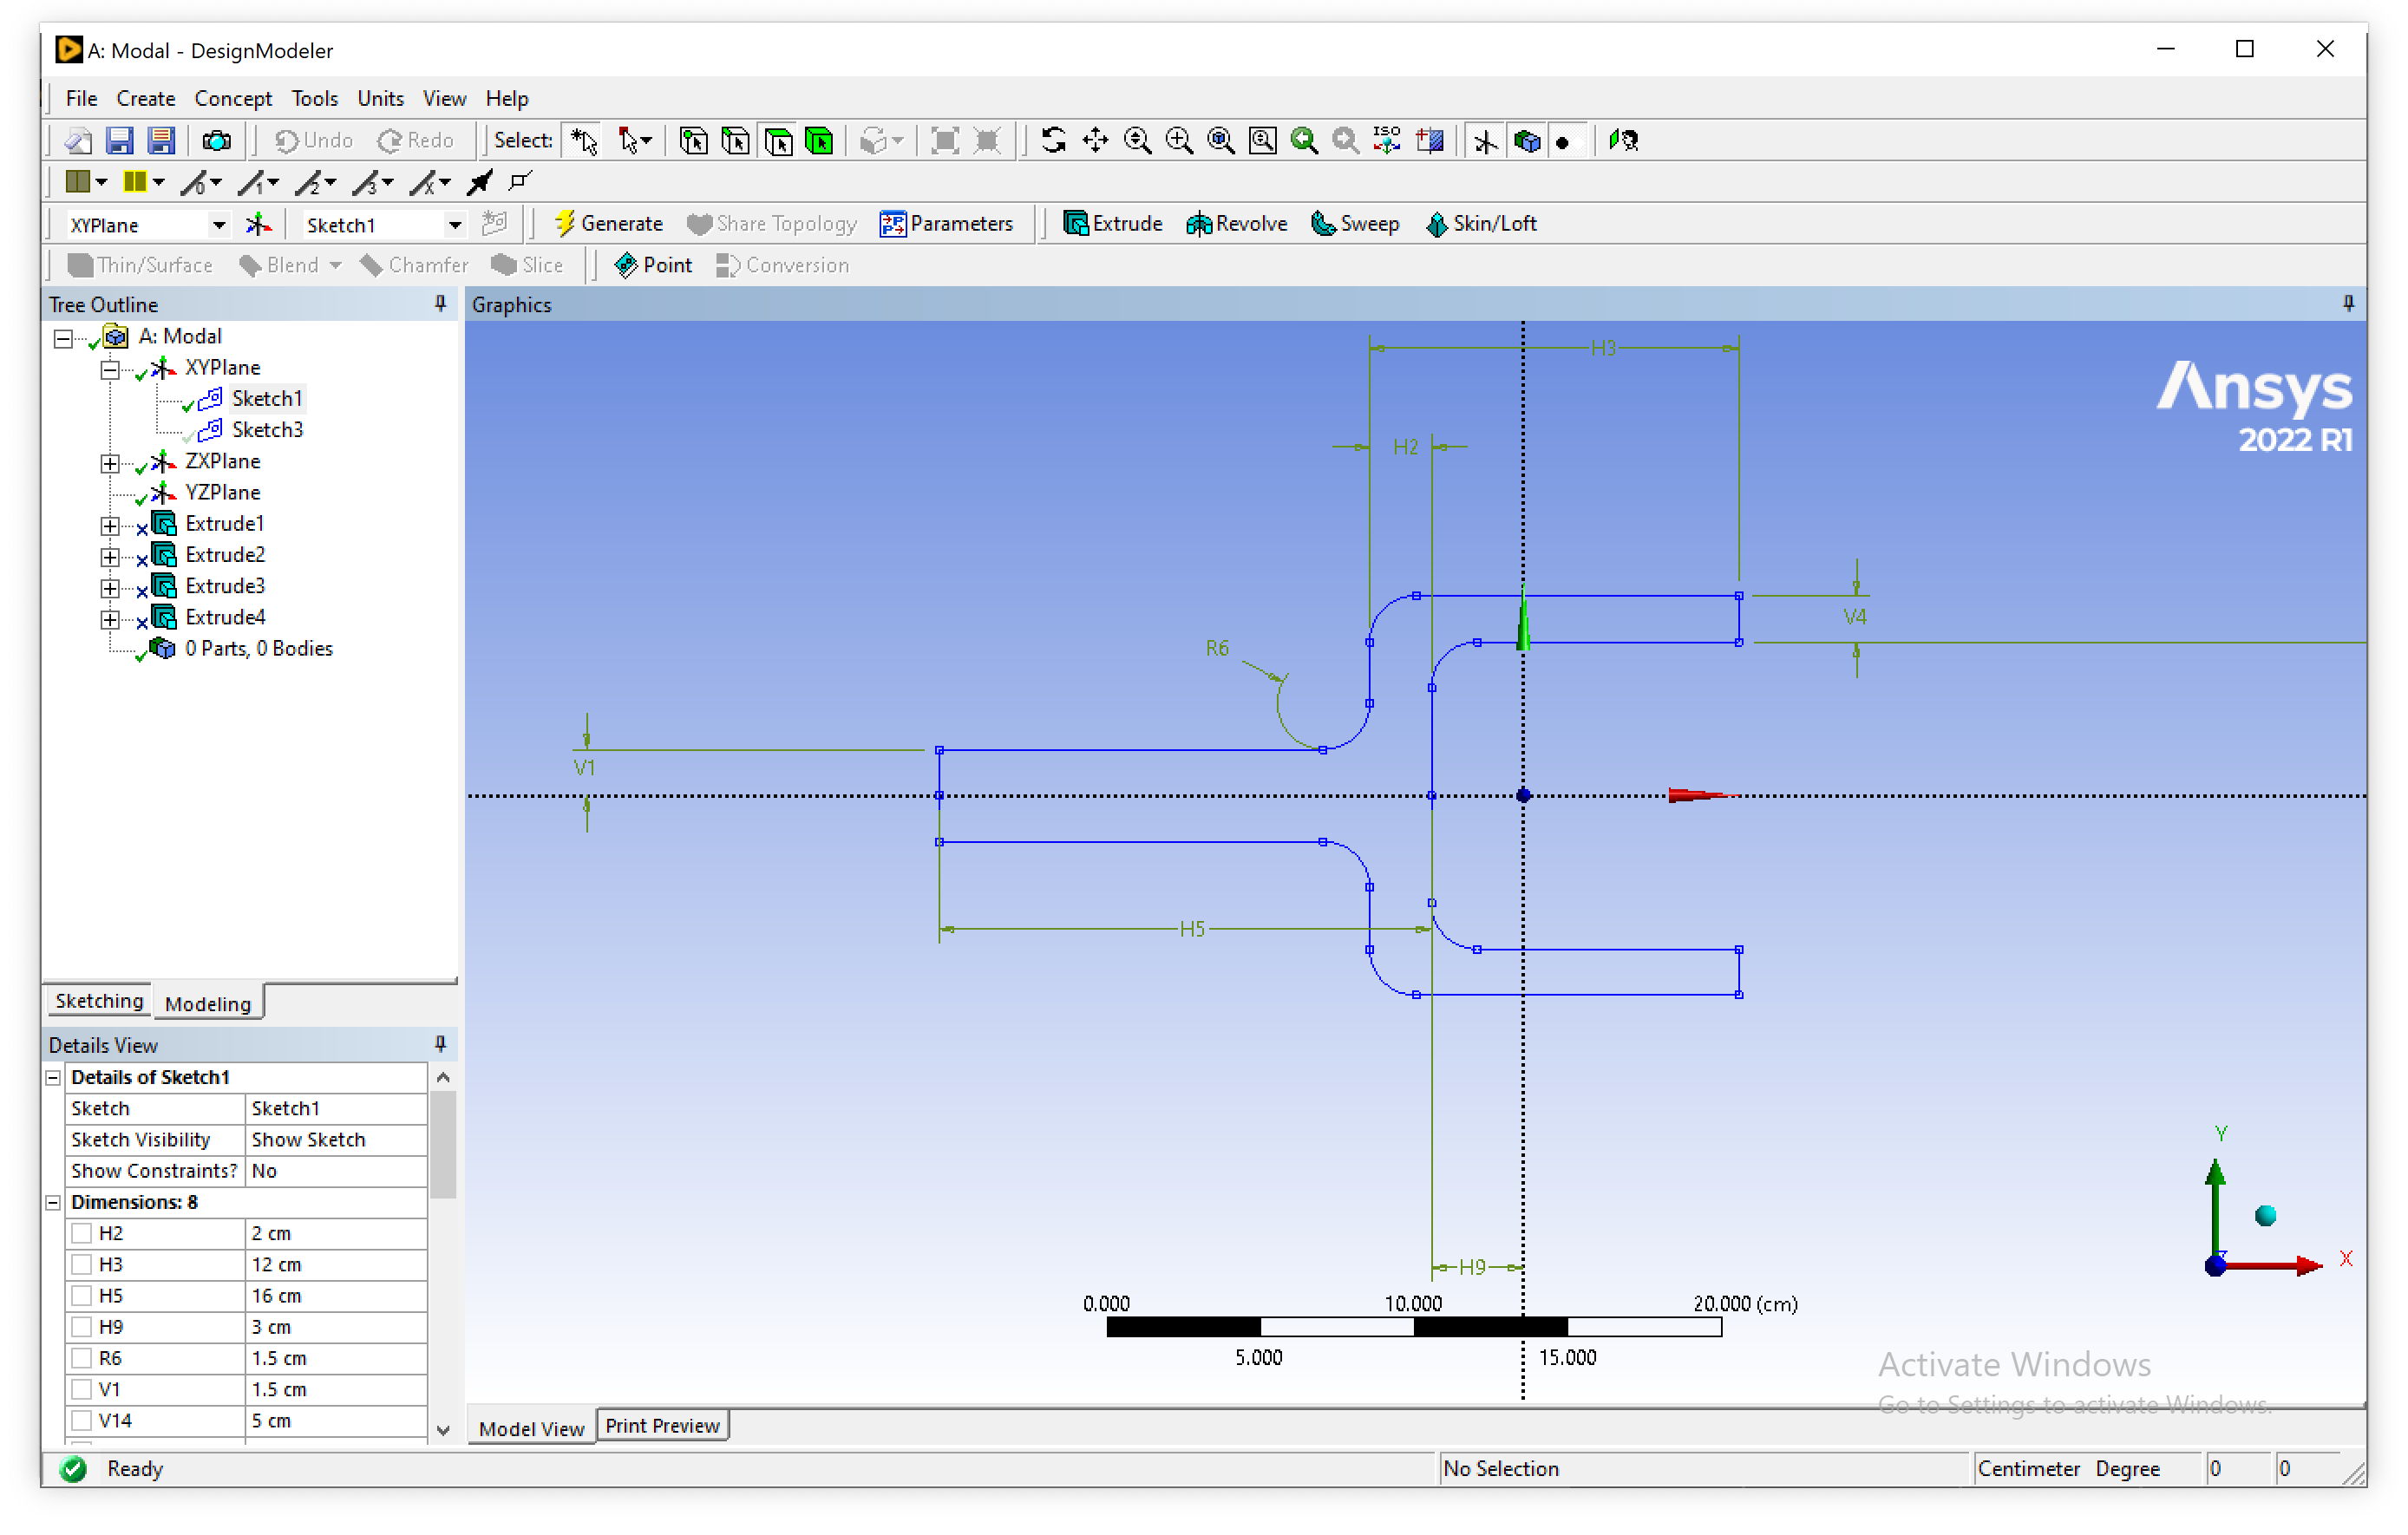
\includegraphics[width=\textwidth]{images/sketch1.png}
	\caption{Эскиз хомута} 
	\label{fig:sketch1}
\end{figure}

После применения функции Extrude из эскиза получаем полноценную 3D деталь-хомут, представленную на рис. \ref{fig:extrude1}.

\begin{figure}[H] 
	\center
	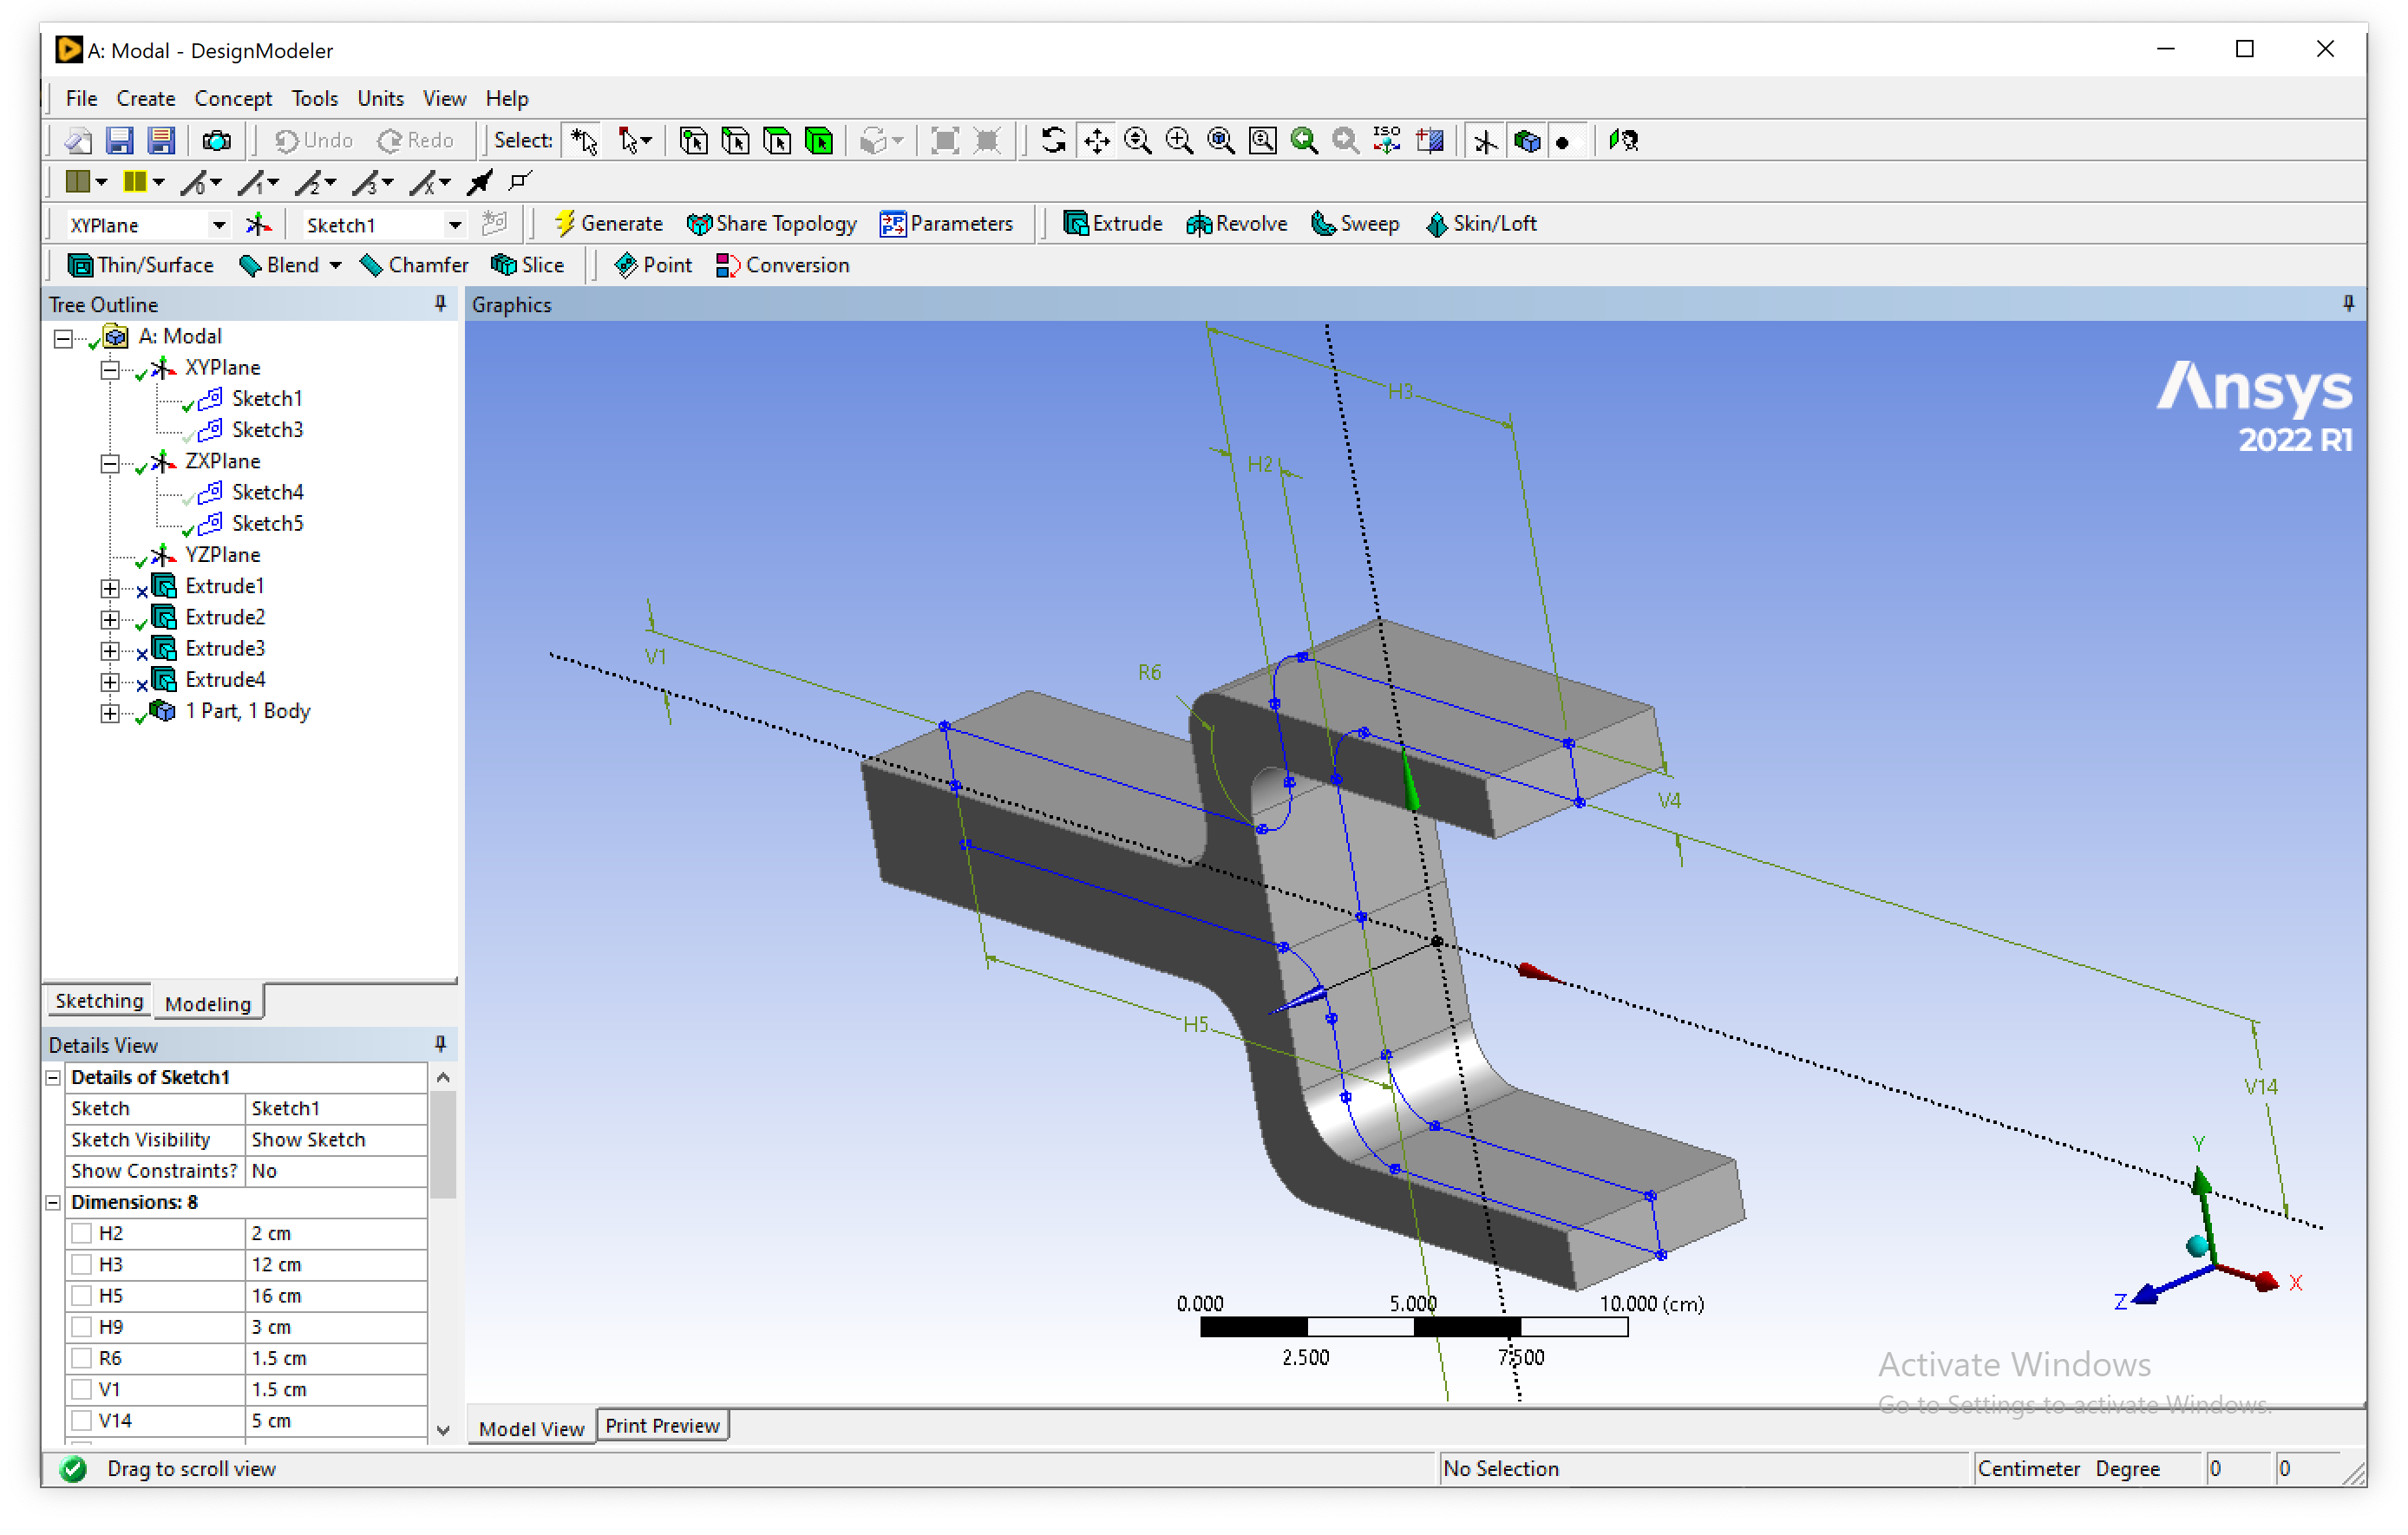
\includegraphics[width=\textwidth]{images/extrude1.png}
	\caption{Деталь-хомут} 
	\label{fig:extrude1}
\end{figure}

На рис.\ref{fig:sketch2} представлен эскиз U-формы.

\begin{figure}[H] 
	\center
	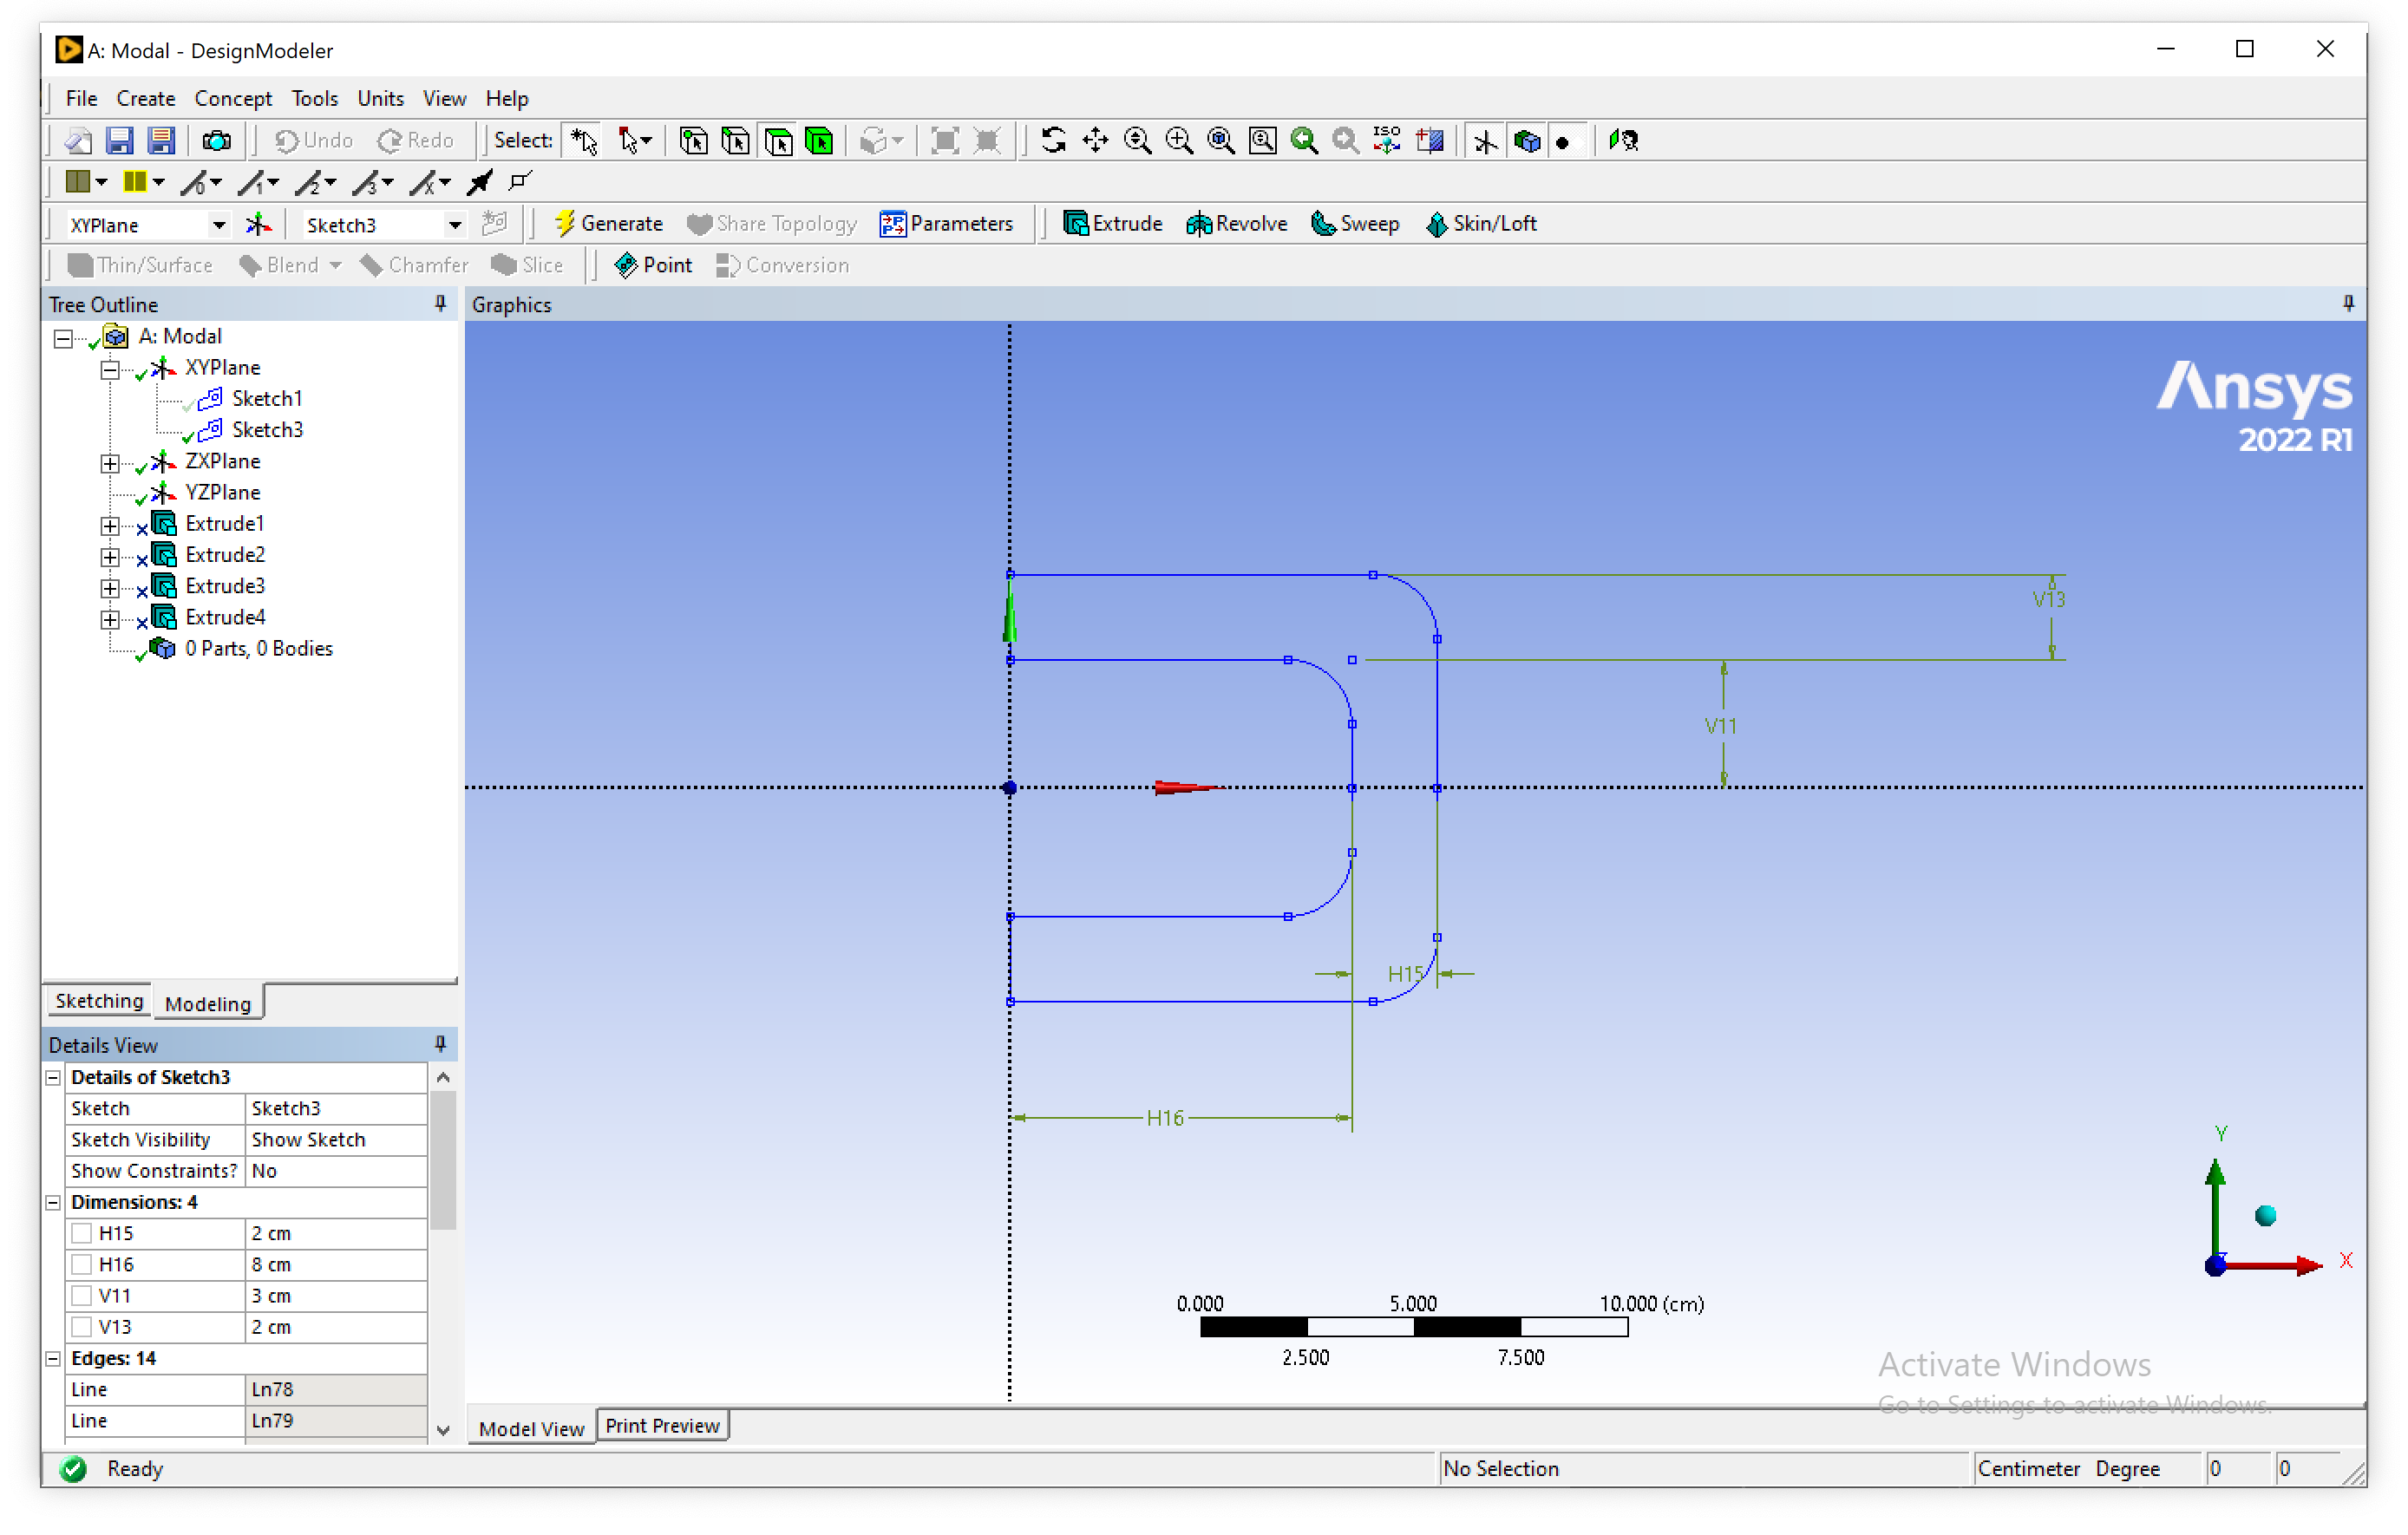
\includegraphics[width=\textwidth]{images/sketch2.png}
	\caption{Эскиз U-формы} 
	\label{fig:sketch2}
\end{figure}

После применения функции Extrude из эскиза получаем полноценную 3D деталь U-формы, представленную на рис. \ref{fig:extrude2}. Ключевые размеры всех деталей указаны в левом нижнем углу соответствующих изображений.

\begin{figure}[H] 
	\center
	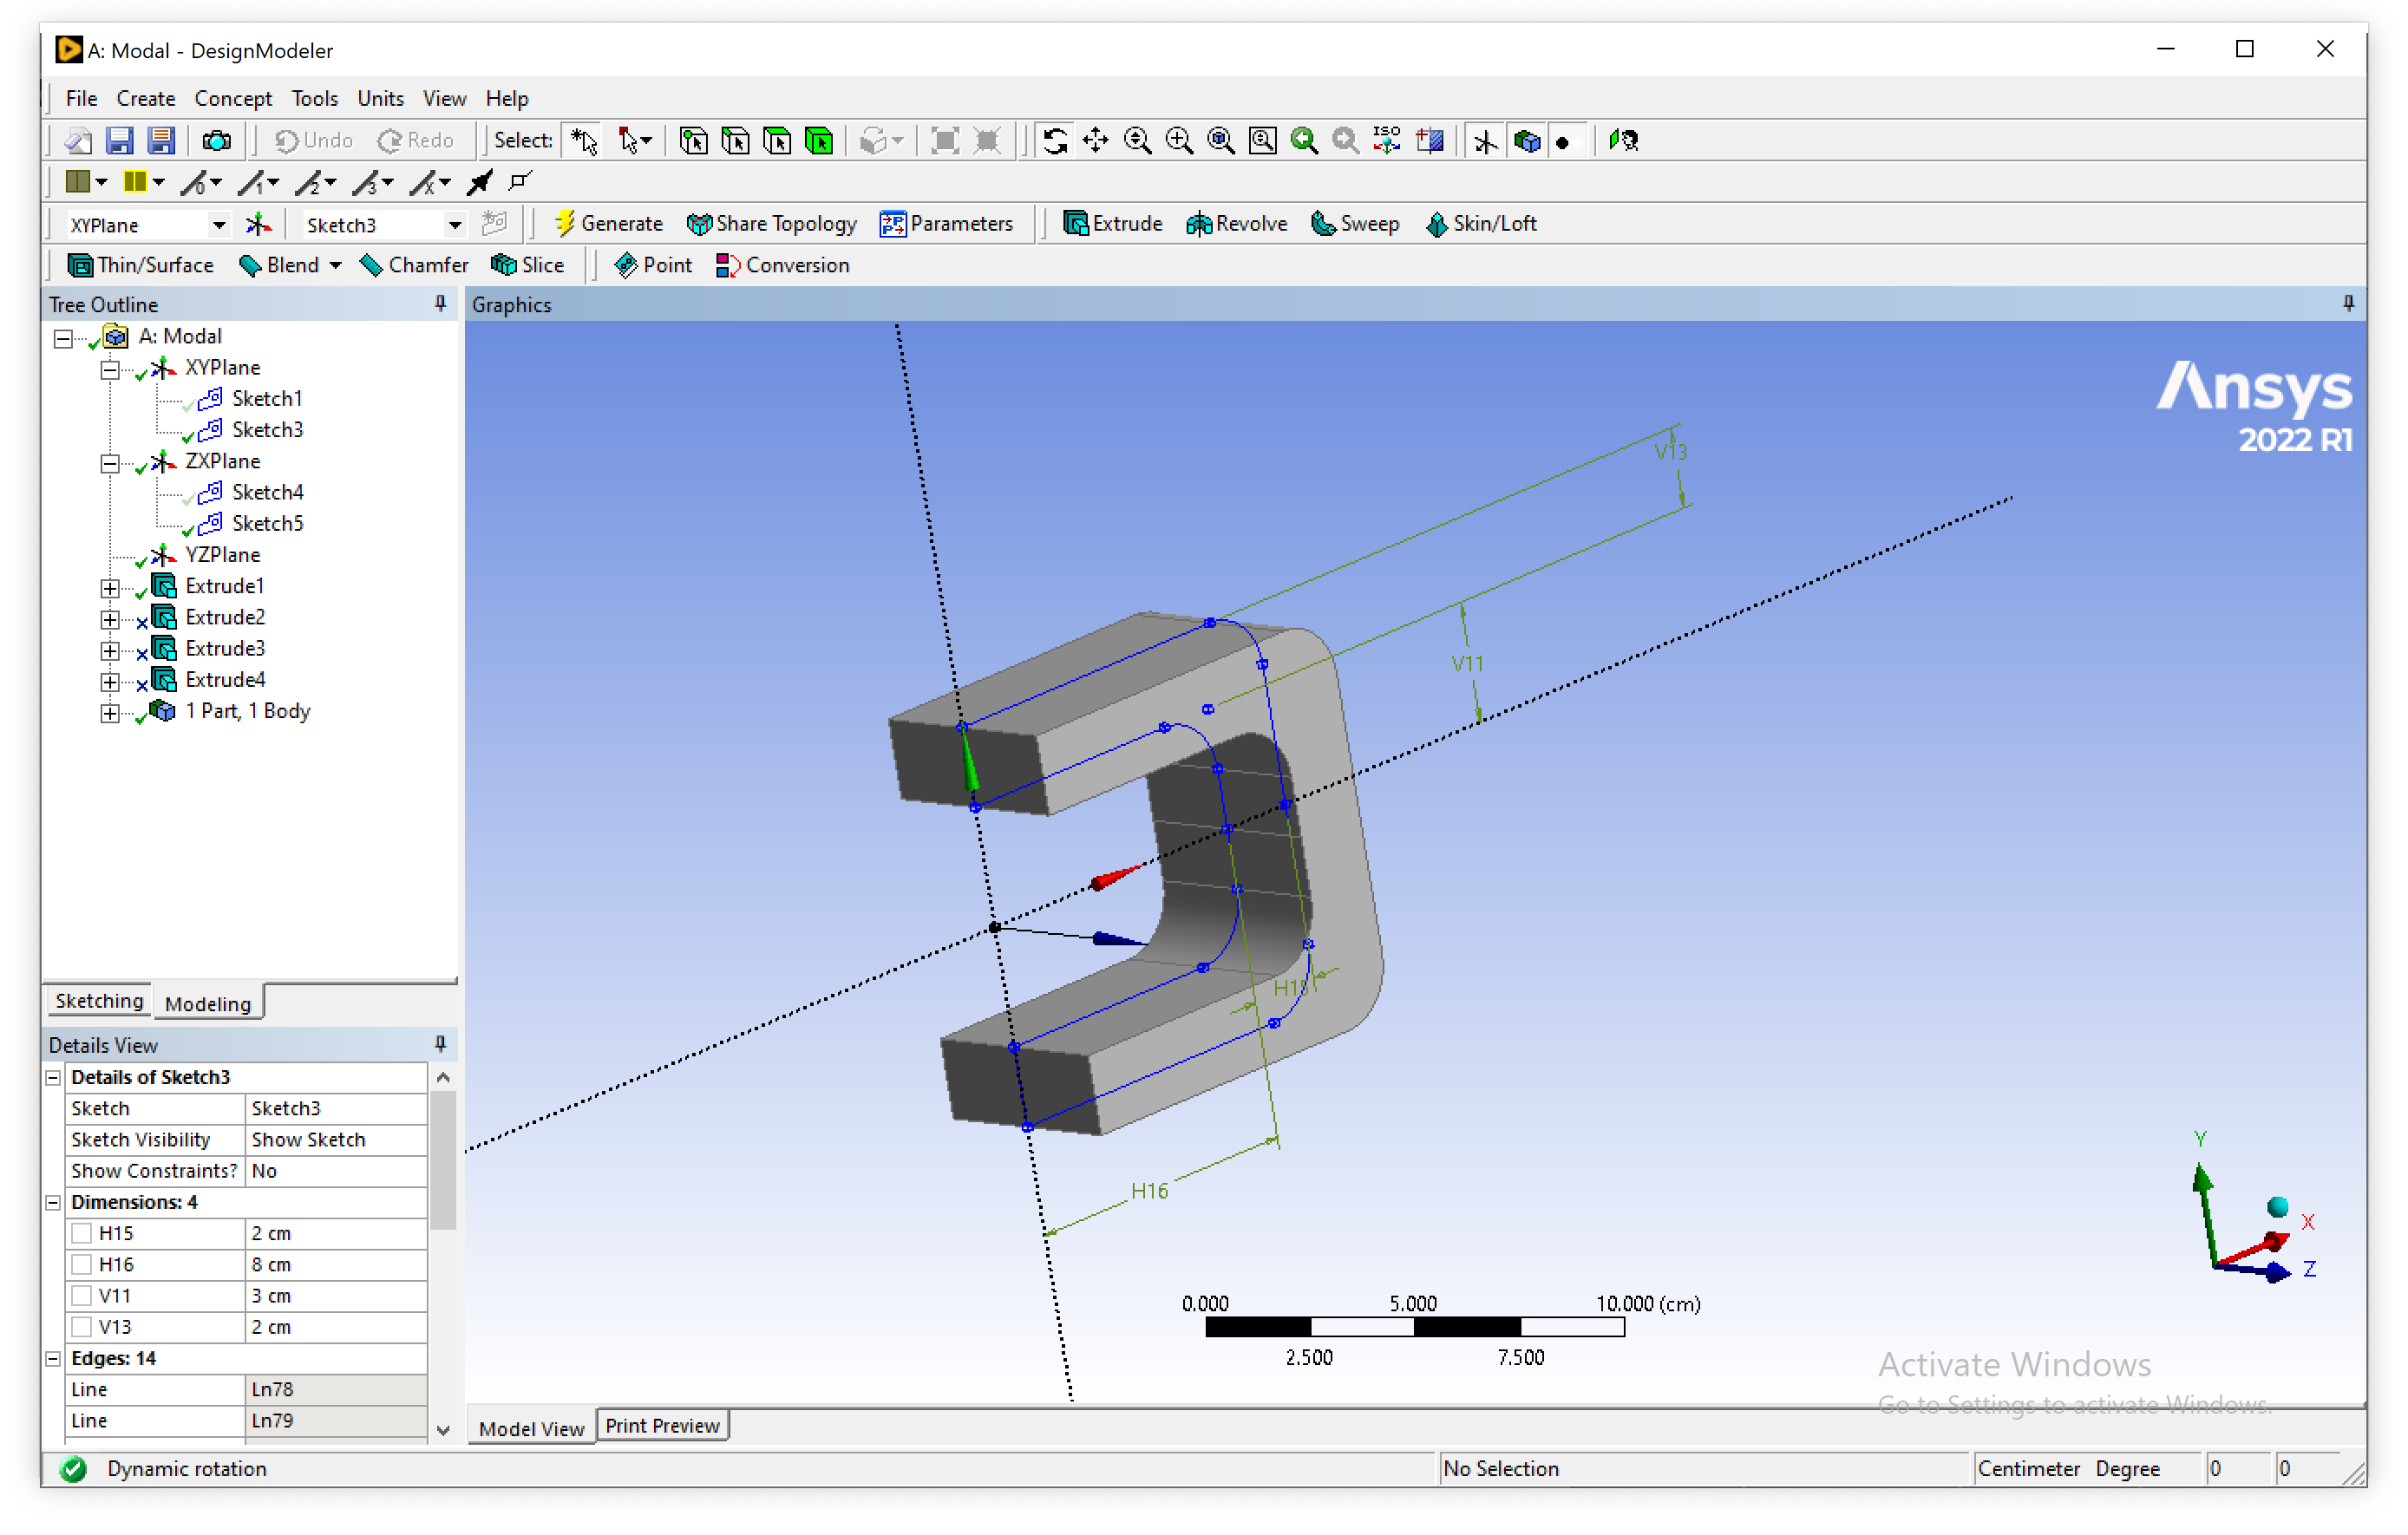
\includegraphics[width=\textwidth]{images/extrude2.png}
	\caption{Деталь U-формы}
	\label{fig:extrude2}
\end{figure}

Далее удаляем часть материала построенных ранее деталей, чтобы в дальнейшем добавить цилиндрическую булавку.

Удаление материала производим с помощью функции Extrude, но теперь с опцией Cut Material. Extrude применяем к новому эскизу, расположенному в плоскости xOz и представляющему из себя круг заданного радиуса.

Дополнительно в опциях объекта Extrude указываем Direction: Both-Symmetric, чтобы удаление материала было успешно проведено по обе стороны от плоскости xOz.

Деталь-хомут и деталь U-формы после удаления части материала (создания цилиндрических отверстий) изображены на рис. \ref{fig:cutmaterial}. Основные опции выполненного Extrude представлены в левом нижнем углу.

\begin{figure}[H] 
	\center
	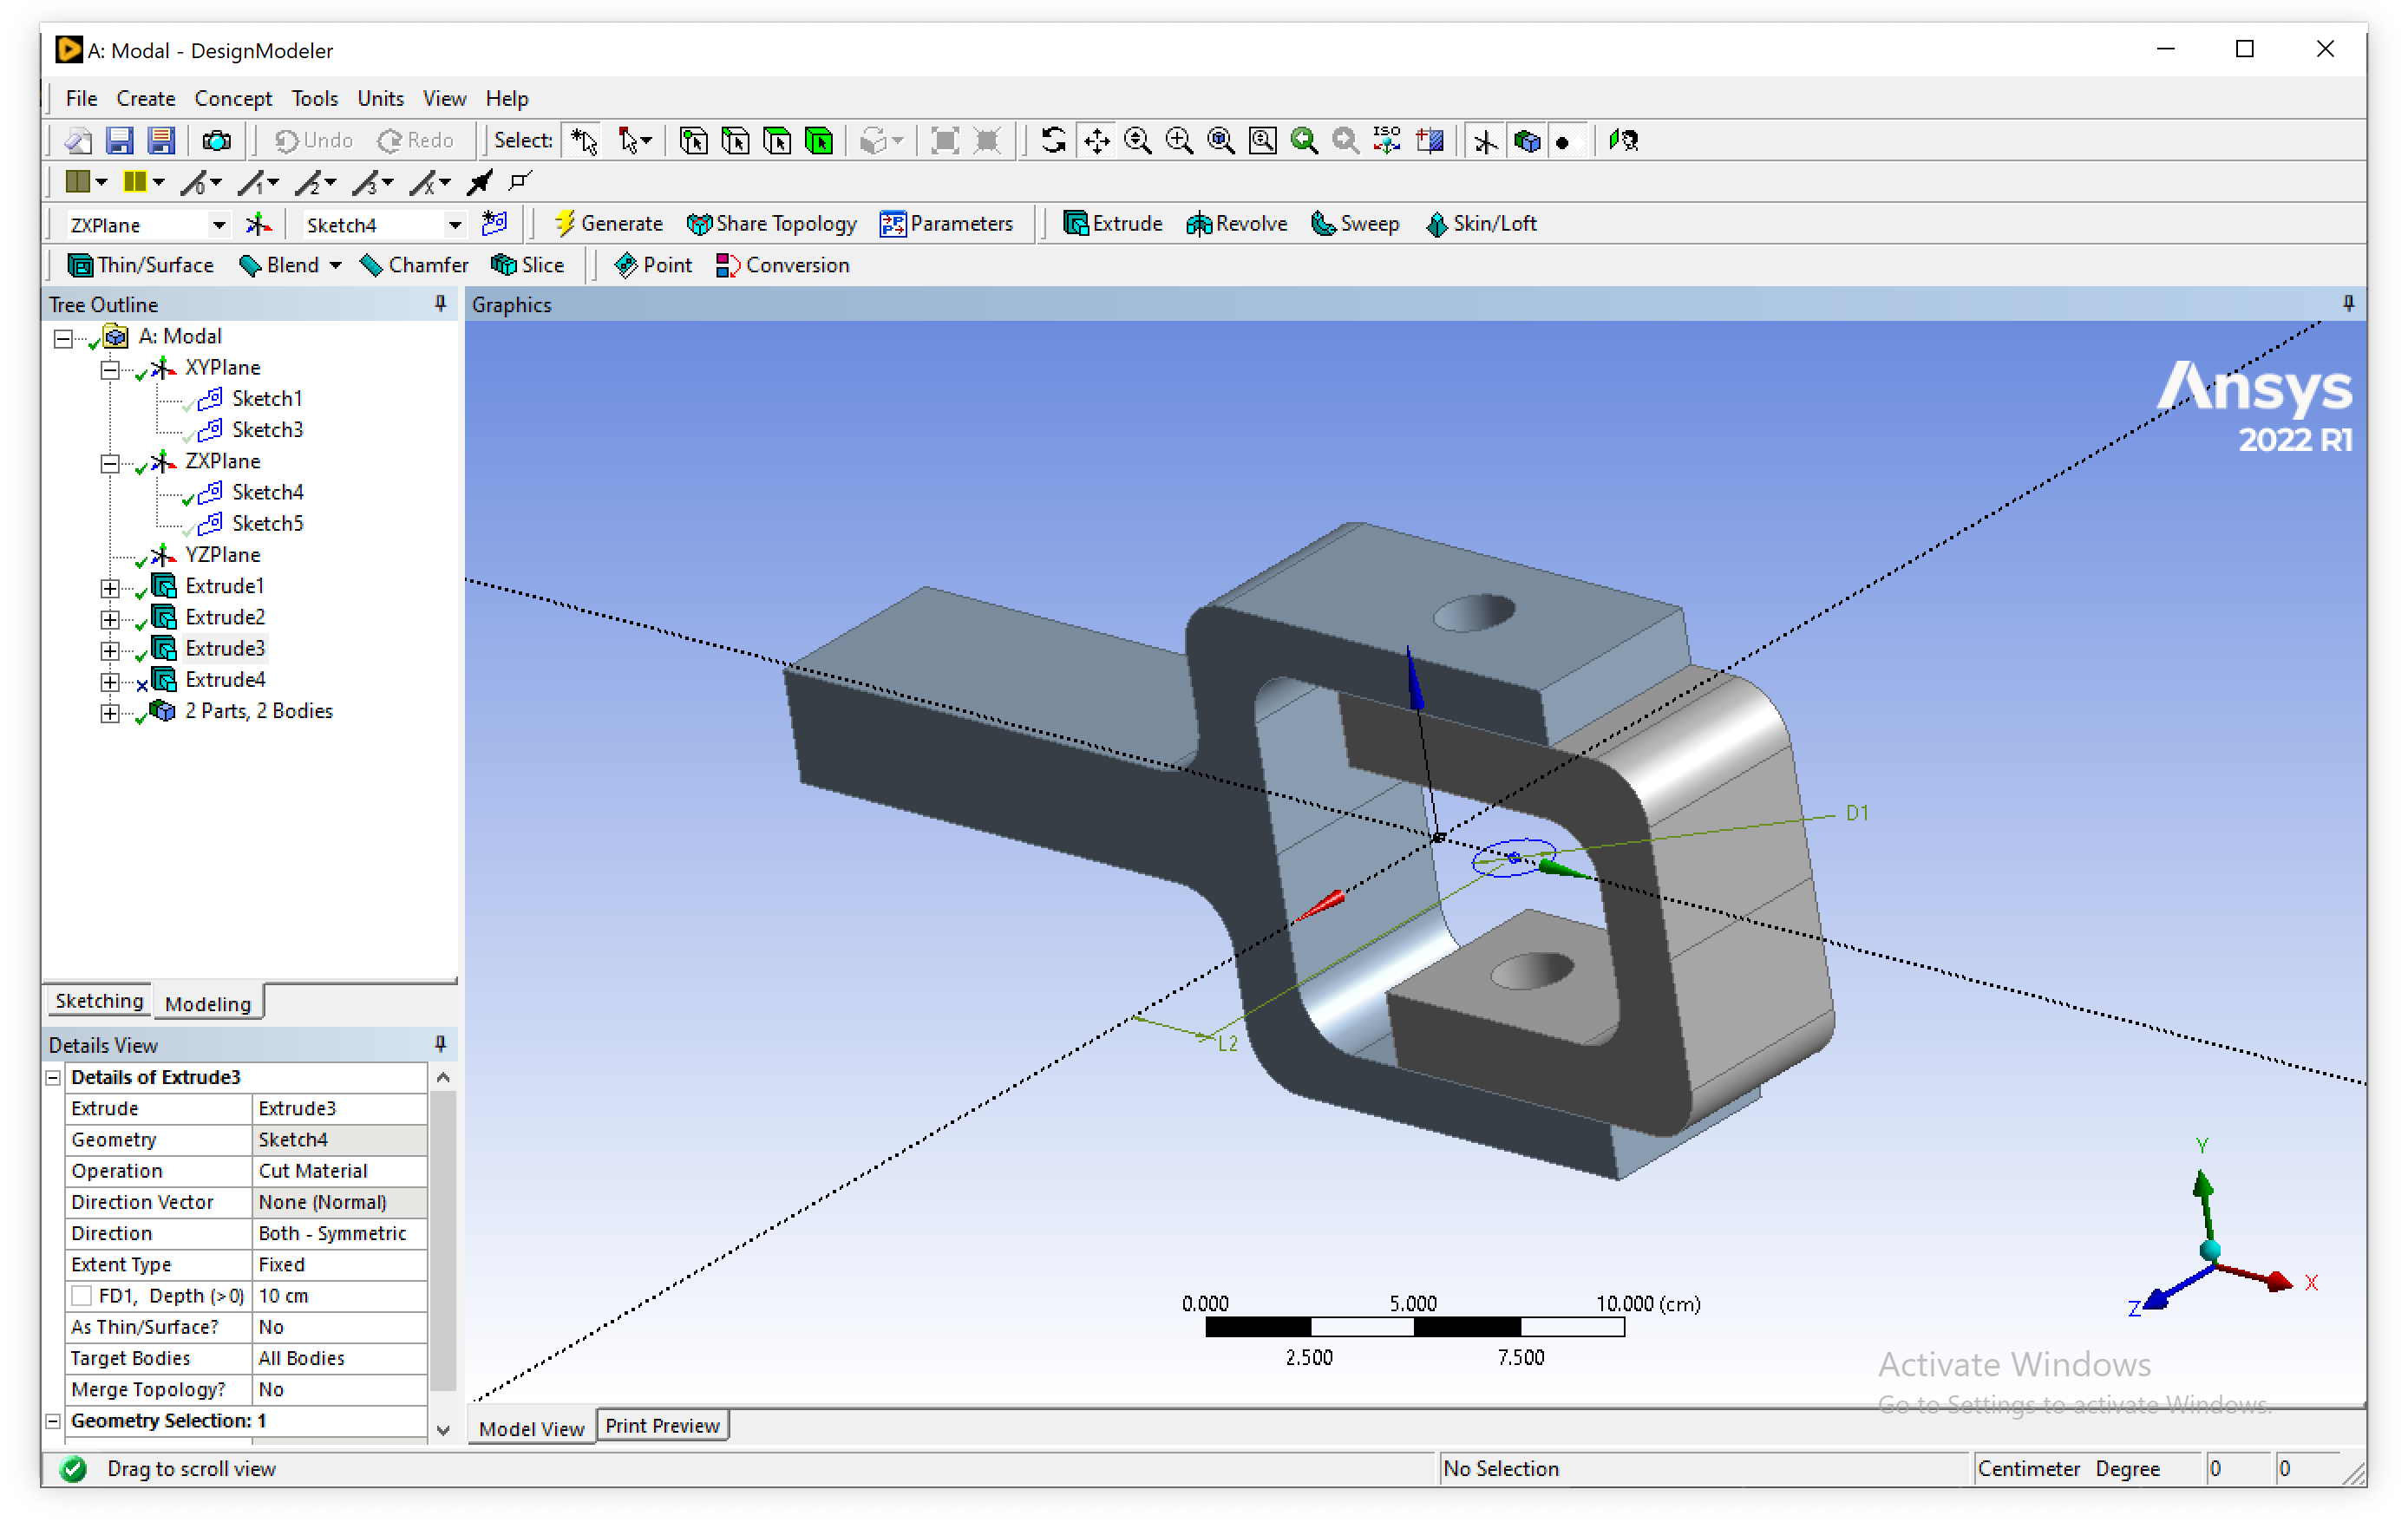
\includegraphics[width=\textwidth]{images/cutmaterial.png}
	\caption{Детали с цилиндрическим отверстием}
	\label{fig:cutmaterial}
\end{figure}

И в завершение построения CAD-модели добавляем цилиндрическую булавку (рис. \ref{fig:extrude3}), скрепляющую ранее построенные детали.

\begin{figure}[H] 
	\center
	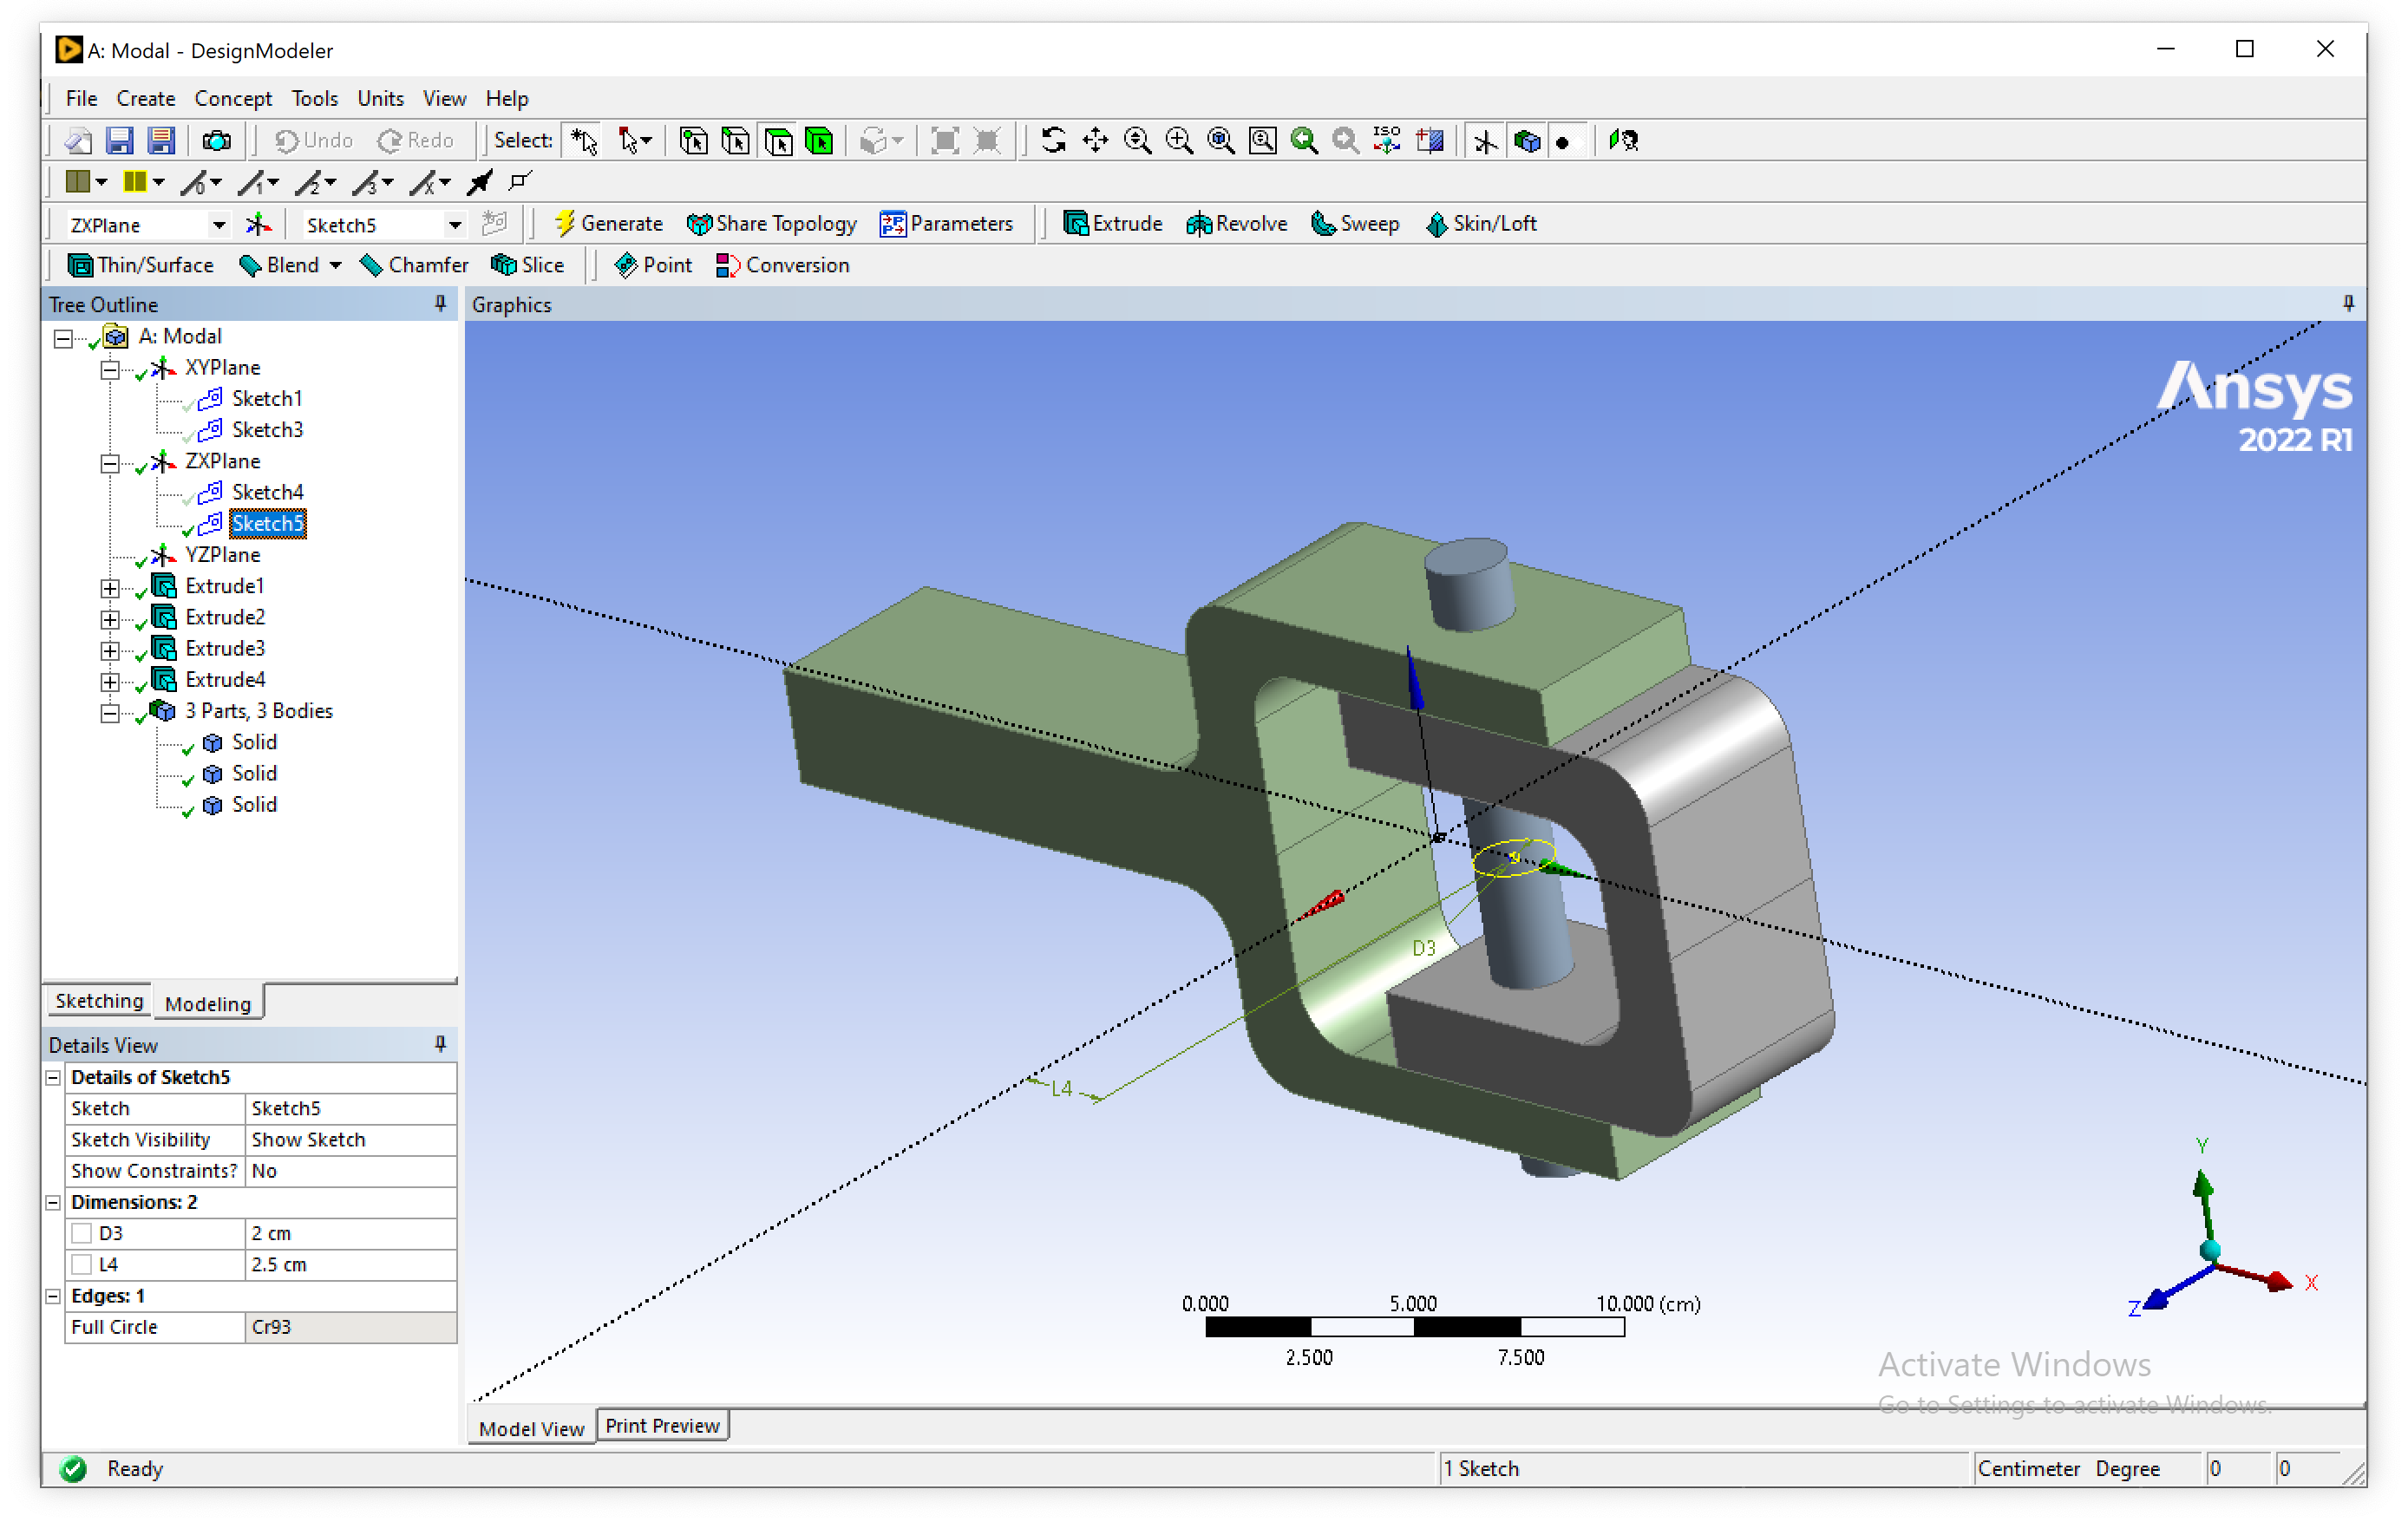
\includegraphics[width=\textwidth]{images/extrude3.png}
	\caption{Добавлена цилиндрическая булавка}
	\label{fig:extrude3}
\end{figure}

Суммарно в процессе построения CAD-модели рассматриваемого изделия были использованы следующие инструменты Ansys DesignModeler: SketchingDrawPolyline (для построения половины эскиза), ModifyFillet (для скругления углов), ModifyReplicate (для симметричного копирования половины эскиза с целью построения полного эскиза), DimensionsHorizontal (для задания горизонтальных размеров эскиза), DimensionsVertical (для задания вертикальных размеров эскиза), DimensionsRadius (для задания радиусов скруглений на эскизе), ConstraintsCoincident (для привязки двух симметричных частей эскиза друг к другу), ConstraintsSymmetry (для задания симметрии частей эскиза относительно оси абсцисс), FlipVertical (для зеркального отображения второй части каждого из эскизов относительно первой части), Extrude (для построения 3D деталей на основе построенных эскизов).

\section{Построение сетки} \label{ch2:sec2}

Конечно-элементную сетку строим с помощью инструментов Ansys Meshing: Face Sizing, Face Meshing и Inflation. На рис. \ref{fig:mesh} представлена построенная сетка.

\begin{figure}[H] 
	\center
	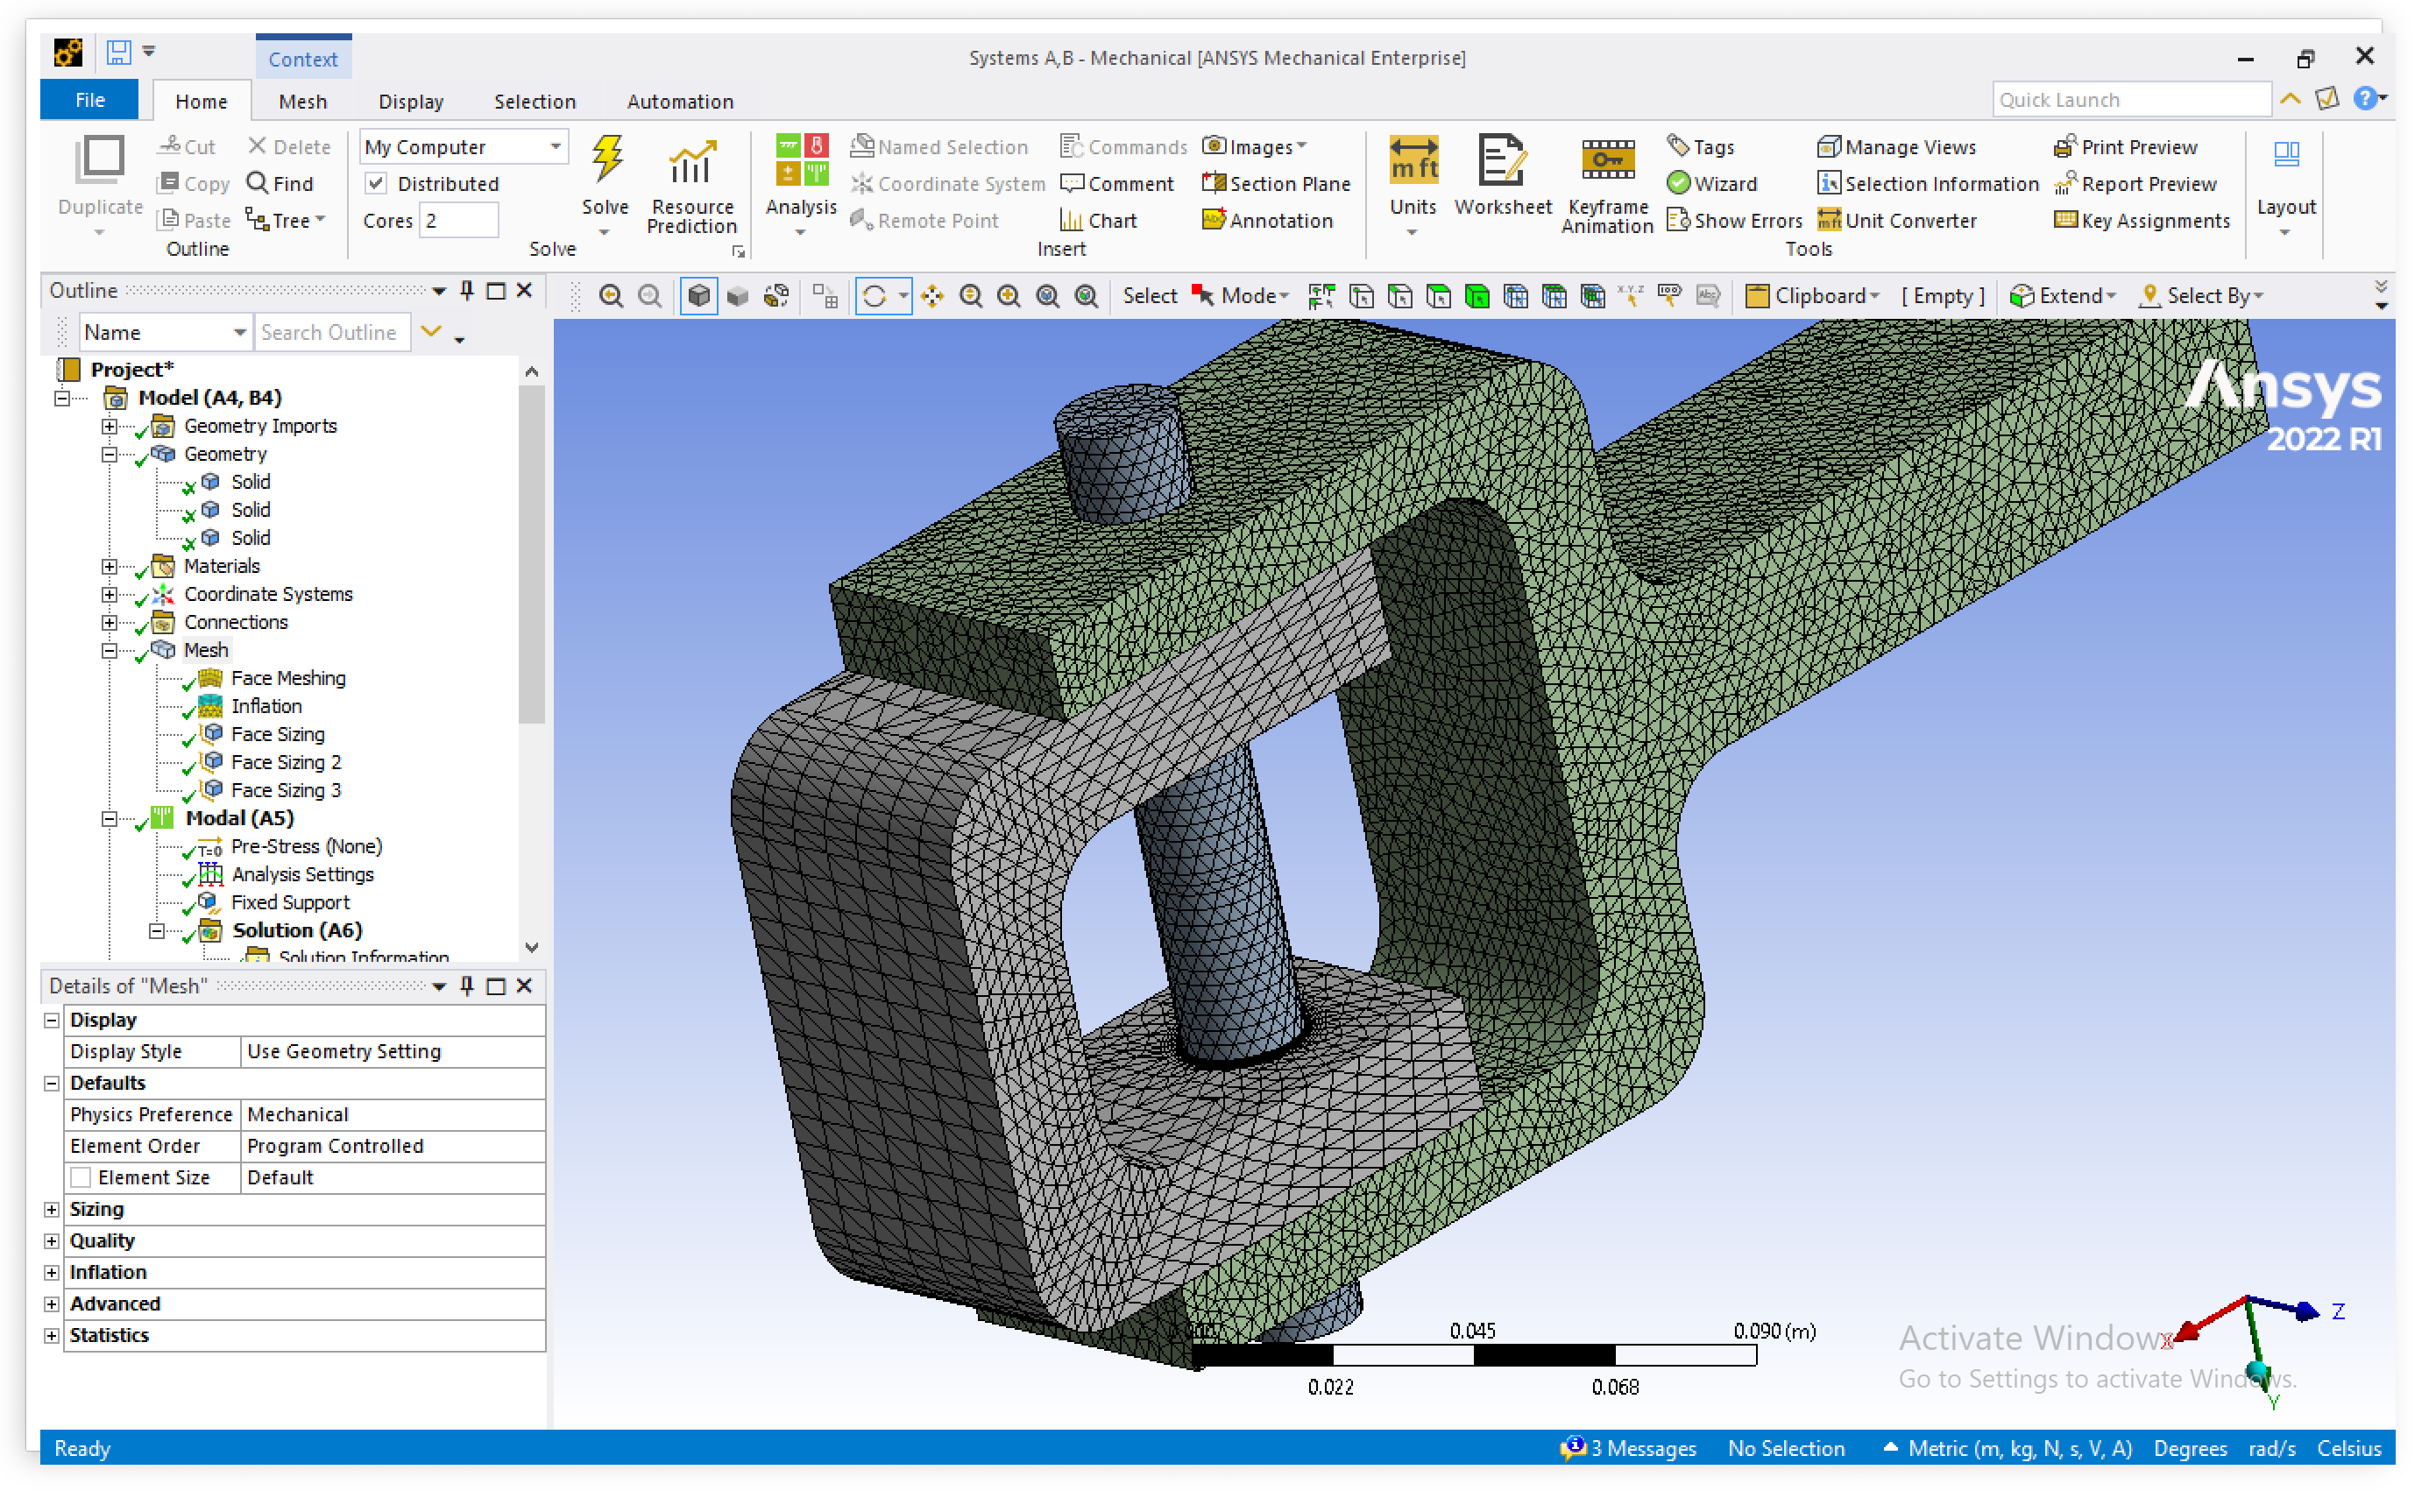
\includegraphics[width=\textwidth]{images/mesh.png}
	\caption{Конечно-элементная сетка}
	\label{fig:mesh}
\end{figure}

В дальнейшем полученная сетка может быть улучшена путём задания только одной специфичной формы элемента сетки и состыковки элементов на границах соседних деталей. Но первоначальный расчёт может быть произведён и на сетке, представленной на рис. \ref{fig:mesh}.

\section{Граничные условия} \label{ch2:conclusion}

На левой стенке хомута задаём условие отсутствия перемещений (рис. \ref{fig:gu}).

\begin{figure}[H] 
	\center
	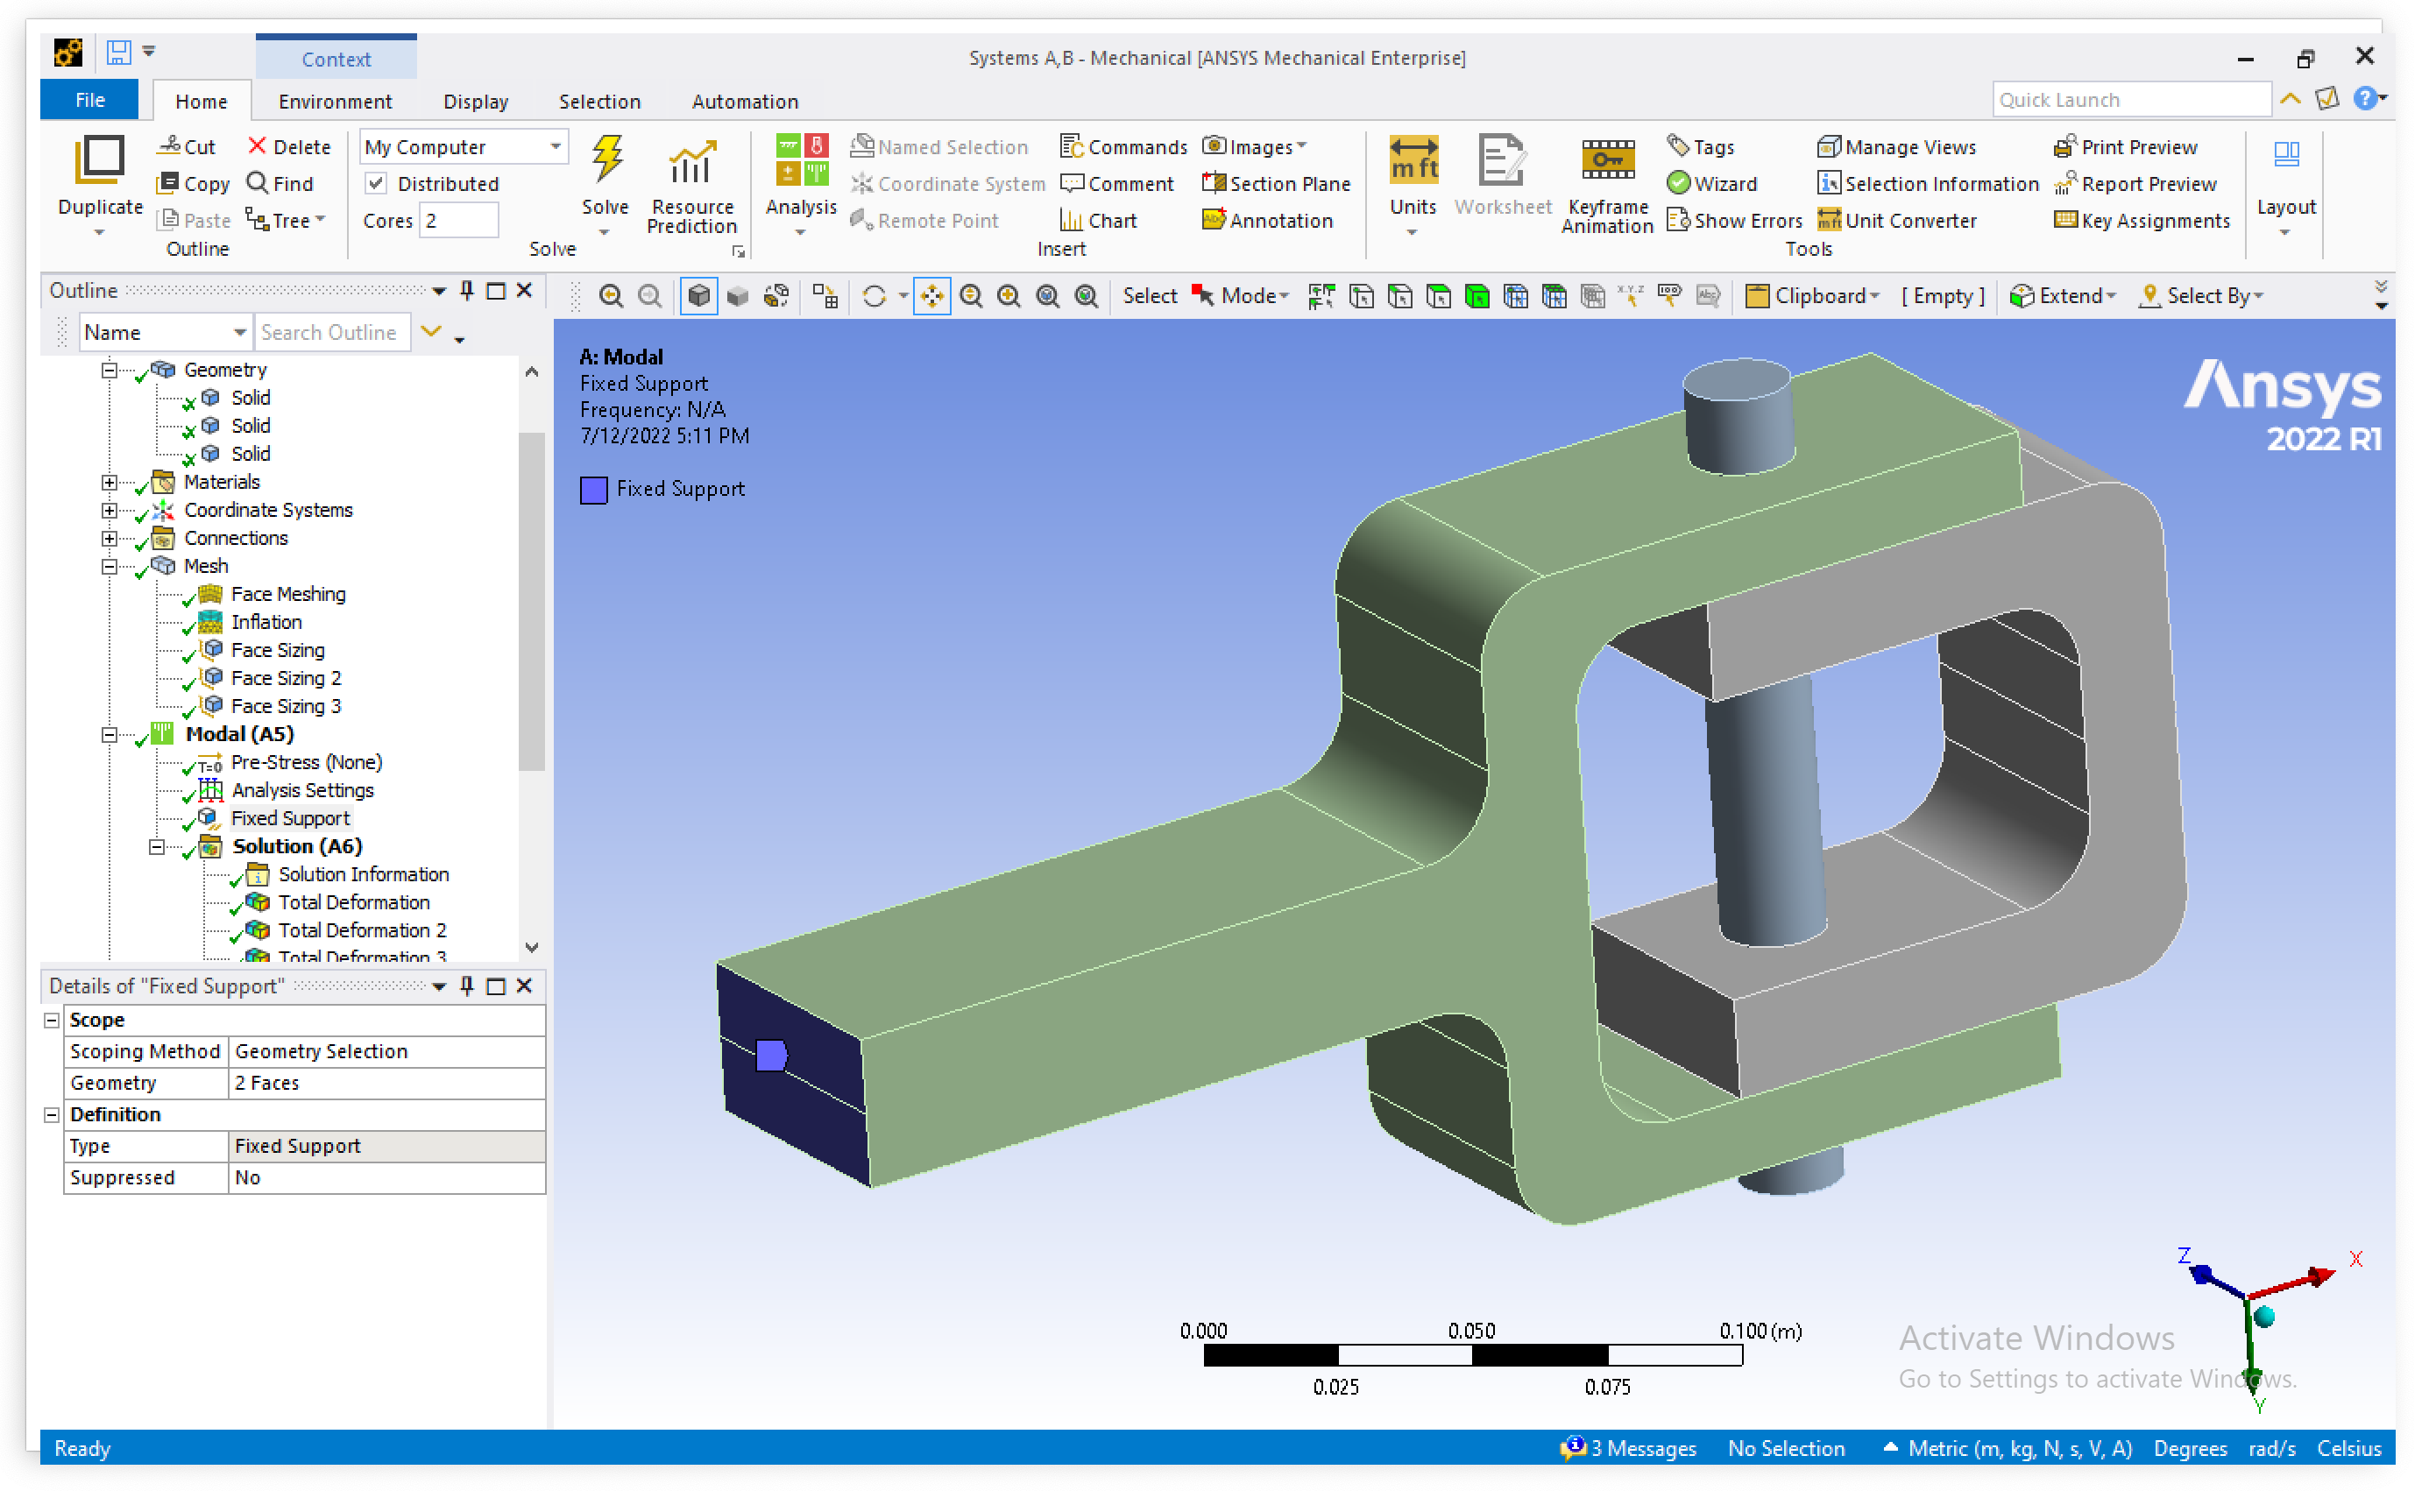
\includegraphics[width=\textwidth]{images/gu.png}
	\caption{Граничное условие (нулевые перемещения)}
	\label{fig:gu}
\end{figure}





